%% Copernicus Publications Manuscript Preparation Template for LaTeX Submissions
%% ---------------------------------
%% This template should be used for copernicus.cls
%% The class file and some style files are bundled in the Copernicus Latex Package which can be downloaded from the different journal webpages.
%% For further assistance please contact the Copernicus Publications at: publications@copernicus.org
%% http://publications.copernicus.org


%% Please use the following documentclass and Journal Abbreviations for Discussion Papers and Final Revised Papers.


%% 2-Column Papers and Discussion Papers
\documentclass[gmd, manuscript]{copernicus}



%% Journal Abbreviations (Please use the same for Discussion Papers and Final Revised Papers)

% Atmospheric Chemistry and Physics (acp)
% Advances in Geosciences (adgeo)
% Advances in Statistical Climatology, Meteorology and Oceanography (ascmo)
% Annales Geophysicae (angeo)
% ASTRA Proceedings (ap)
% Atmospheric Measurement Techniques (amt)
% Advances in Radio Science (ars)
% Advances in Science and Research (asr)
% Biogeosciences (bg)
% Climate of the Past (cp)
% Drinking Water Engineering and Science (dwes)
% Earth System Dynamics (esd)
% Earth Surface Dynamics (esurf)
% Earth System Science Data (essd)
% Fossil Record (fr)
% Geographica Helvetica (gh)
% Geoscientific Instrumentation, Methods and Data Systems (gi)
% Geoscientific Model Development (gmd)
% Geothermal Energy Science (gtes)
% Hydrology and Earth System Sciences (hess)
% History of Geo- and Space Sciences (hgss)
% Journal of Sensors and Sensor Systems (jsss)
% Mechanical Sciences (ms)
% Natural Hazards and Earth System Sciences (nhess)
% Nonlinear Processes in Geophysics (npg)
% Ocean Science (os)
% Primate Biology (pb)
% Scientific Drilling (sd)
% SOIL (soil)
% Solid Earth (se)
% The Cryosphere (tc)
% Web Ecology (we)



%% \usepackage commands included in the copernicus.cls:
%\usepackage[german, english]{babel}
%\usepackage{tabularx}
%\usepackage{cancel}
%\usepackage{multirow}
%\usepackage{supertabular}
%\usepackage{algorithmic}
%\usepackage{algorithm}
%\usepackage{float}
%\usepackage{subfig}
%\usepackage{rotating}

\usepackage{amsmath}
 

\begin{document}

%\linenumbers

\title{SED (1.0): A new, numerically efficient sediment module for the coupling to Earth System Models}


% \Author[affil]{given_name}{surname}
\Author[1]{Dominik}{H\"ulse}
\Author[1]{Sandra}{Arndt}
\Author[2]{Stuart}{Daines}
\Author[1, 3]{Andy J.}{Ridgwell}

\affil[1]{School of Geographical Sciences, University of Bristol, Clifton, Bristol BS8 1SS, UK}
\affil[2]{Earth System Science, University of Exeter, North Park Road, Exeter EX4 4QE, UK}
\affil[3]{Department of Earth Sciences, University of California, Riverside, CA 92521, USA}

%% The [] brackets identify the author with the corresponding affiliation. 1, 2, 3, etc. should be inserted.



\runningtitle{SED (1.0)-a sediment modle for Earth System Models}

\runningauthor{Arndt et al.}

\correspondence{Sandra Arndt (s.arndt@bristol.ac.uk)}



\received{}
\pubdiscuss{} %% only important for two-stage journals
\revised{}
\accepted{}
\published{}

%% These dates will be inserted by Copernicus Publications during the typesetting process.


\firstpage{1}

\maketitle



\begin{abstract}
TEXT
\end{abstract}



\introduction  %% \introduction[modified heading if necessary]
Role of marine sediments for climate and global biogeochemical cycles\\
Diagenetic Models\\
How are sediment resolved in Earth System models\\
Problem with that\\
Alternative Model approaches, e.g. from coastal reserach\\
Solution presented here\\ 


\section{Model Description}
This section describes the formulation and solution of the model. A glossary of parameters along with their respective units is provided in Table \ref.

\subsection {General Model Approach} \label{subsec:GeneralModelApproach}
The calculation of benthic return/uptake and burial fluxes is based on the vertically resolved conservation equation for solid and dissolved species in porous media is given by 
\citep[e.g.][]{berner_early_1980, boudreau1997diagenetic}:

\begin{equation} 
\frac{\partial \xi C_i}{\partial t}=-\frac{\partial F}{\partial z}+\xi \sum_j R_i^j \label{eq:Eq_generaldiagenetic}
\end{equation}

where $C_i$ is the concentration of the biogeochemical species $i$, $\xi$ equals the porosity $\phi$ for solute species and $(1-\phi)$ for solid species, hence represents the partitioning of species $i$ 
into the solute and dissolved phase. The term $z$ is the sediment depth, $t$ denotes the time, $F$ summarises the transport fluxes and $\sum_j R_i^j$ represents the sum of production/consumption rates $j$ 
that affect species $i$. The reaction network has to account for the most important primary and secondary redox reactions, equilibrium reactions, mineral dissolution and precipitation, as well as adsorption 
and desorption processes.\\
State-of-the-art reaction-transport models generally solve Eq. (\ref{eq:Eq_generaldiagenetic}) numerically and thus allow to account for transient conditions, depth-varying parameters or a high degree of coupling 
between different chemical species. Yet, numerical models are computational expensive, thus rendering their application in an Earth System Model framework prohibitive. 
An analytical solution of Eq. (\ref{eq:Eq_generaldiagenetic}) provides an alternative and computational more efficient approach. Analytical models enjoyed great popularity in the early days of diagenetic modelling 
due to the low computing power. However, early analytical models were often very problem-specific and only considered one or two coupled species  \textcolor{red}{(e.g. Lehrman, Berner) ?? which pubs?}. 
A number of more complex analytical models describing the coupled dynamics of ....were developed \citep[e.g.][]{billen1982modelling, goloway1982diagenetic, jahnke1982model}. 

Finding an analytical solution to  Eq. (\ref{eq:Eq_generaldiagenetic}), especially when complex reaction networks are to be considered is not straightforward and generally requires the assumption of steady state. 
Because the Earth system model relevant variability in boundary conditions and fluxes is generally longer than the characteristic timescales of the reaction-transport processes, the sediment can be described by a 
series of pseudo steady-states. In addition, the complexity of the reaction network can be reduced by dividing the sediment into distinct zones and accounting for the most pertinent biogeochemical processes 
within each zone, thus increasing the likelihood of finding an analytical solution to Eq. (\ref{eq:Eq_generaldiagenetic}). The model divides the sediment into a bioturbated and a non-bioturbated zone 
defined by the constant bioturbation depth $z_{bio}$. In addition, it accounts for the dynamic redox zonation of marine sediments by dividing the sediment into: 2) an oxic zone situated between the 
SWI and a dynamically calculated penetration depth of oxygen $z_{O_2}$, 3) a denitrification zone situated between $z_{O_2}$ and a dynamically calculated penetration depth of nitrate $z_{NO_3}$, 4) 
a sulfate reduction zone situated between $z_{NO_3}$ and a dynamically calculated penetration depth of sulfate $z_{SO_4}$and 5) a methanogenic zone situated below $z_{SO_4}$ (Figure \ref{fig:Sediment_layers}). 
Each zone is characterised by a set of diagenetic equations that encapsulate the most pertinent reaction and transport processes in the respective zone (see section \ref{sec:transport} and \ref{sec: ReactionNetwork} 
form more detail). 
\begin{figure}[htbp]
\begin{center}
	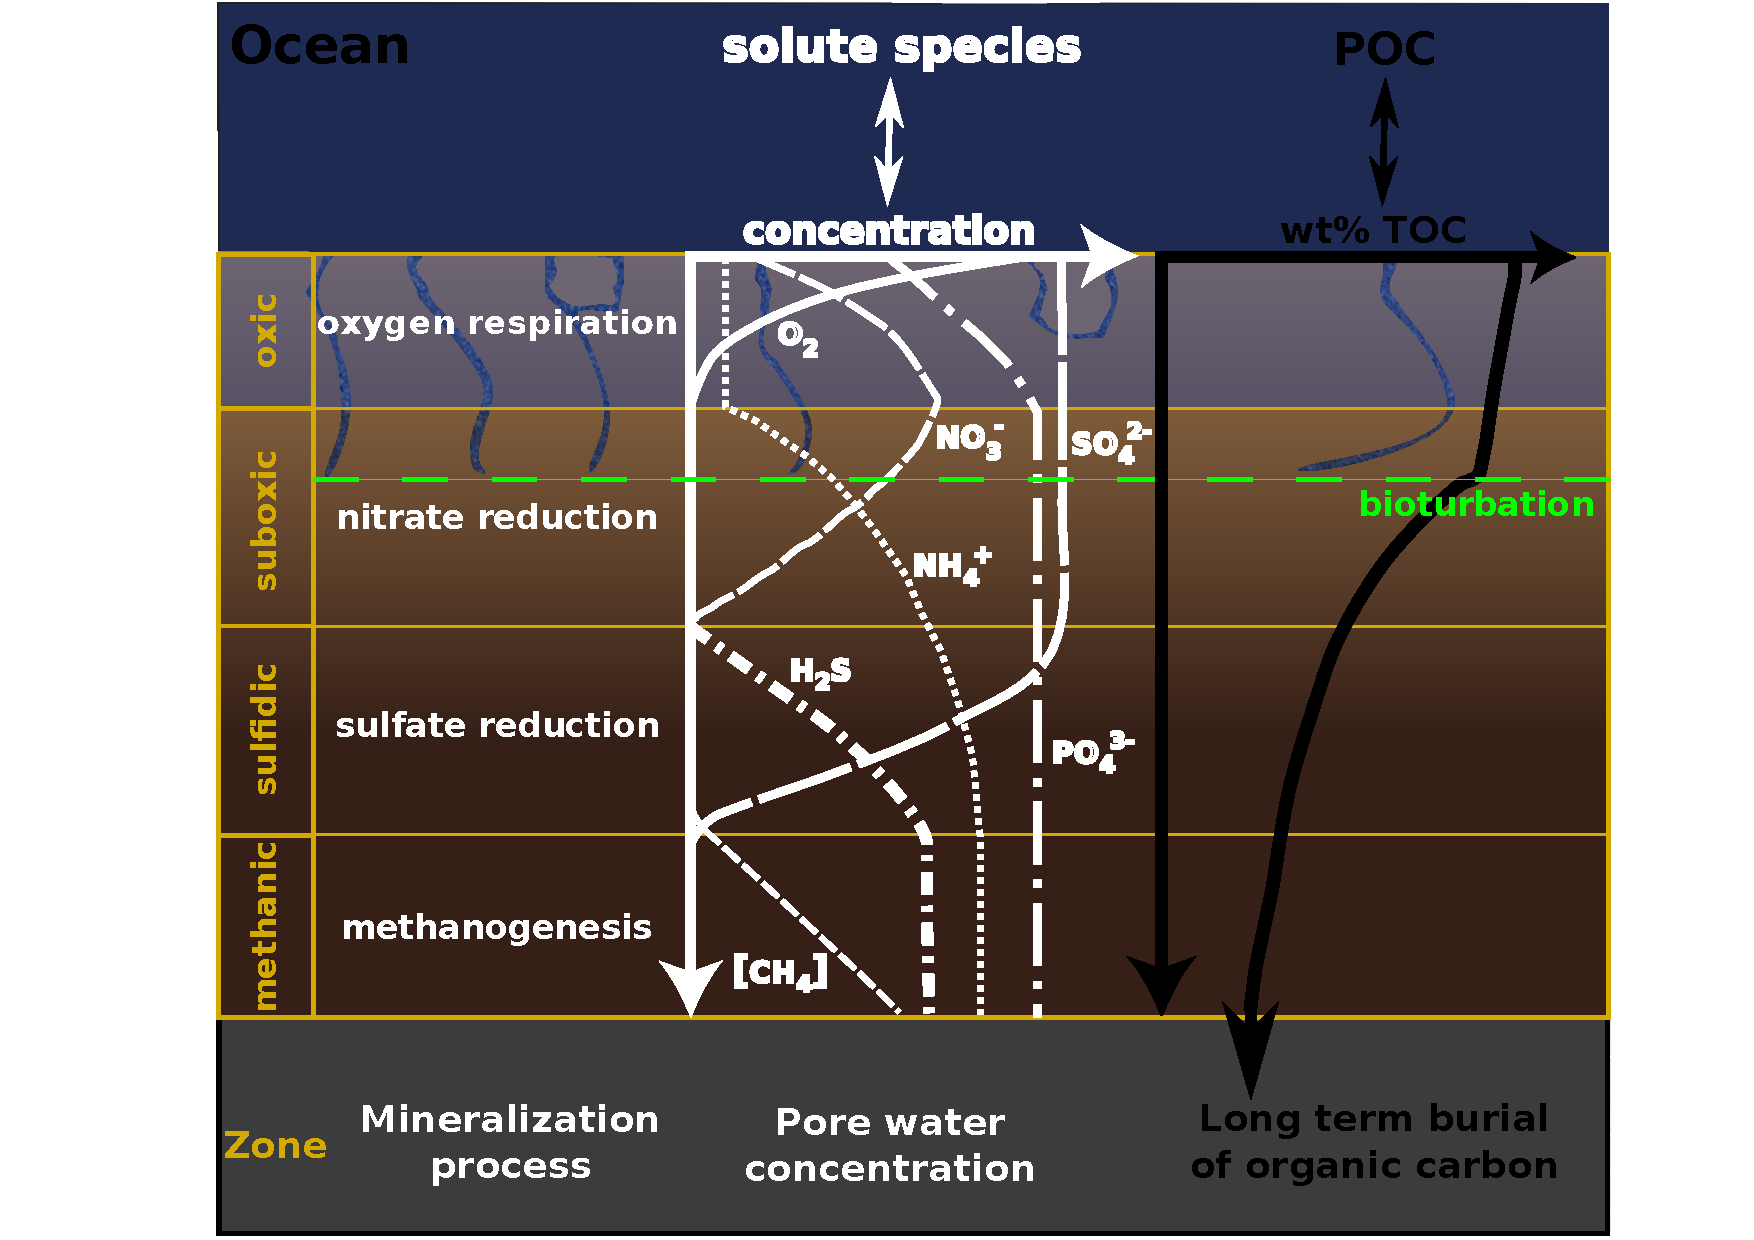
\includegraphics[width=0.8\textwidth]{figures/Sediment-model-with-profiles-rotated90.pdf}
	\caption{Schematic of the different modelled species and layers in our sediment model. Here showing the case $z_{ox} < z_{bio} < z_{NO_3} < z_{SO_4}$.}
	\label{fig:Sediment_layers}
	\end{center}
\end{figure}

\subsection{Transport}
The model accounts for both advection and diffusion of dissolved and solid species, assuming that sediment compaction is negligible ($\frac{\partial \phi}{\partial z}$=0). 
The diffusion of dissolved species is described via an apparent diffusion coefficient, $D_{i0}$. In addition, the activity of infaunal organisms in the bioturbated zone of the sediment ($z<z_{bio}$) causes random 
displacements of sediments and porewaters and is simulated using a diffusive term (e.g. Boudreau,1986), with a constant bioturbation coefficient $D_{bio}$ in the bioturbated zone. 
The pumping activity by burrow-dwelling animals, the so-called bioirrigation, is encapsulated in a factor, $f_{ir}$ that enhances the molecular diffusion coefficient, 
$D_{mol,i}$ \citep[ hence, $D_{i,0}=D_{mol,i}\cdot f_{ir}$,][]{soetaert1996dynamic}.  The divergence of the flux is thus given by:
\begin{equation}
\frac{\partial F}{\partial z}=-\frac{\partial}{\partial z}\left( -\xi D_i \frac{\partial C_i}{\partial z} +\xi w C_i\right) \label{Eq_flux_divergence}
\end{equation}
where $D_i$ is the diffusion coefficient of species $i$ ($D_i=D_{i,0}+D_{bio}=D_{mol,i}\cdot f_{ir}+D_{bio}$ for dissolved species and $D_i=D_{bio}$ for solid species) and $w$ is the burial rate. 
The bioturbation coefficient $D_{bio}$ is set to zero below $z_{bio}$. In addition, infaunnal activity ceases ($D_{bio}=0$) once bottom waters become anoxic (O$_2$ = 0.0 mol cm$^{-3}$ ). 
\textcolor{red}{last bit not like that in model}


\subsection{Reaction Network}
Earth System models generally track the evolution of the global biogeochemical cycles of organic and inorganic carbon, the essential nutrients (nitrogen, phosphorus) and oxygen with the aim of investigating the evolution 
of the ocean's redox structure and carbonate system and its feedbacks on global climate. This general aim thus defines a minimum set of state variables and reaction processes that need to be resolved for an efficient 
representation of the benthic-pelagic coupling in Earth System Models. The sediment model has to provide robust quantifications of organic and inorganic carbon burial fluxes, growth-limiting nutrient, equilibrium invariant 
and reduced species return fluxes, and oxygen uptake fluxes. As a consequence, the reaction network must explicitly or implicitly account for the most important primary and secondary redox reactions, equilibrium reactions, 
mineral precipitation/dissolution and adsorption/desorption, resulting in a complex set of coupled reaction-transport equations. The following 
subsections provide a short discussion of the reaction processes included in the model and table \ref{tab_reactions} \textcolor{red}{what to do here?} provides an overview of the vertically resolved conservation equations for solid and dissolved species 
in each layer.

\subsubsection{Organic matter}
In marine sediments, organic matter (OM) is degraded by heterotrophic activity coupled to the sequential utilisation of terminal electron acceptors (TEAs), typically in the order of O$_2$, NO$_3^-$, Mn(VI), Fe(III) and SO$_4^{2-}$ 
followed by methanogenesis and/or fermentation. Organic matter degradation is described via a multi-G model approach \citep[][and references therein]{arndt_quantifying_2013}, assuming that the bulk OM is divided 
into discrete compound classes $C_i$ characterised by specific degradation rate constants $k_i$. Such a multi-G approach allows for selective preservation of compound classes according to their degradability, $k_i$ and, thus, accounts 
for the change in organic matter degradability with burial. Each compound class is degraded according to first-order kinetics. Organic matter dynamics are thus described by:

\begin{equation}
 \frac{\partial C_i}{\partial t} = 0= D_{C_i} \frac{\partial^2C_i }{\partial z^2} - w\frac{\partial C_i }{\partial z} - k_i\cdot C_{i} \label{eq:ODE_OC}
\end{equation}
where:
\begin{align}
 D_{C_i}&=D_{bio} 	 &\text{if ($z\leq z_{bio}$)}\\
 D_{C_i}&=0            &\text{if ($z > z_{bio}$)} 
\end{align}
The solution of Eq. \ref{eq:ODE_OC} (see section \ref{sec:Solution} for details) requires the definition of boundary conditions. The model assumes a known concentration/flux at the sediment-water interface and continuity 
across the bottom of the bioturbated zone, $z_{bio}$ (Table \ref{Tab:BC_OM+O2}).
\begin{table}[tbp]
\caption{Boundary conditions for organic matter and oxygen.}
% title of Table
\centering
% used for centering table
\begin{tabular}{ |l| l| l|}
\hline
\textbf{Boundary}& \textbf{Condition}&\\
\hline
$z=0$& known concentration& 1) $C_i(0)=C_{i0}$  \\
$z=z_{bio}$&continuity& 2) $C_i(z_{bio}^-)$=$C_i(z_{bio}^+)$\\
               &&3) $D_{bio}\cdot \frac{\partial C_i}{\partial z}|_{z_{bio}^-}=0$\\
%Dom was               &&3) $D_{bio}\cdot \frac{\partial C_i}{\partial z}|_{z_{bio}^-}-w\cdot C_i(z_{bio}^-)=-w\cdot C_i(z_{bio}^+)$\\
\hline
$z=0$& known concentration& 1) $O_2(0)=O_{20}$  \\
$z=z_{bio}$&continuity& 2) $O_2(z_{bio}^-)$=$O_2(z_{bio}^+)$\\
               &&3) $\left(D_{O_2,0}+D_{bio}\right )\cdot \frac{\partial O_2}{\partial z}|_{z_{bio}^-}=D_{O_2,0} \cdot \frac{\partial O_2}{\partial z}|_{z_{bio}^+}$\\
%Dom was               &&3) $\left(D_{bio}+D_{mol,O_2}\right )\cdot \frac{\partial O_2}{\partial z}|_{z_{bio}^-}-w\cdot O_2(z_{bio}^-)=D_{mol,O_2} \cdot \frac{\partial O_2}{\partial z}|_{z_{bio}^+}-w\cdot O_2(z_{bio}^+)$\\
$z=z_{ox}$& $O_2$ consumption& 4)$ O_2(z_{ox})=0$ \quad or \quad $\frac{\partial O_2}{\partial z}|_{z_{ox}}=0$\\
$z=z_{ox}$& Flux from below& 5) $-\omega D_{O_2} \cdot \frac{\partial O_2}{\partial z}|_{z_{ox}}=F_{red, z_{ox}}$\\   
&with:\textcolor{red}{ correct? \&}&$ \quad F_{red,z_{ox}}=\frac{1-\phi}{\phi} \cdot \int_{z_{ox}}^{\infty}  \sum_i \left( 2\gamma_{NH_4} NC_i + \delta SC_i \right) k_i C_i\ dz$ \\
&\textcolor{red}{why $\omega$ at 5) (delete!?)}&\\
% was from Sandra &with:&$F_{red,z_{ox}}=\beta \cdot \int_{z_{ox}}^{\inf}  \sum_i k_i\cdot C_i  dz  + 2\cdot \gamma \cdot \int_{z_{O_2}}^{\inf}  \sum_i k_i\cdot C_i  -  $ \\
\hline    
\end{tabular}
\label{Tab:BC_OM+O2}
% is used to refer this table in the text
\end{table}


\subsubsection{Oxygen}
Oxygen serves as the most powerful terminal electron acceptor for the heterotrophic degradation of organic carbon. In addition, the oxidation of reduces species produced through microbial activity throughout the 
sediment column further contributes to the consumption of oxygen. The model explicitly accounts for the consumption of oxygen by heterotrophic degradation and nitrification of ammonium in the oxic layer of the sediment. 
In addition, the oxygen consumption through the oxidation of reduced species (Fe$^{2+}$, Mn$^{2+}$, NH$_4$, H$_2S$) produced in the suboxic and anoxic layers of the sediment is implicitly taken into account through the flux 
boundary condition at the dynamic oxygen penetration depth $z_{ox}$. This simplification can be justified as it has been shown that these secondary redox reactions mainly occur at the oxic/suboxic interface \citep{soetaert_model_1996}.  
Oxygen is described in $mol\ cm^{-3}$ liquid and conversion from the solid phase of mineralized organic matter (expressed in $mol\ cm^{-3}$ bulk sediment) to consumption of dissolved oxygen (or later nutrients) introduce 
a factor of $\frac{1-\phi}{\phi}$, where $\phi$ is the sediment porosity. Oxygen dynamics are thus described by:
\begin{align} 
 \frac{\partial O_2}{\partial t} &= 0= D_{O_2}\frac{\partial^2 O_2 }{\partial z^2} - w\frac{\partial O_2}{\partial z} - \frac{1-\phi}{\phi}\sum_i k_i \cdot [ OC + 2 \gamma_{NH_4} NC_i ]\cdot C_{i}(z) \label{eq:ODE_O2_1}
\end{align}
where:
\begin{align}
 D_{O_2}&=D_{O_2, 0}+D_{bio}  &\text{if ($z\leq z_{bio}$)}\\
 D_{O_2}&=D_{O_2, 0}                &\text{if ($z > z_{bio}$)} 
\end{align}  
To solve Eq. \ref{eq:ODE_O2_1} analytically (see section \ref{sec:Solution}) boundary conditions at three depths are defined (Table \ref{Tab:BC_OM+O2}). 
The model assumes a known bottom water concentration and the complete consumption of oxygen at the oxygen penetration depth (or zero flux if $z_{ox}=z_\infty$). 
It considers equal oxygen concentration and diffusive flux above ($z_{bio}^-$) and 
below ($z_{bio}^+$) the bioturbation boundary. In addition, the model imposes a flux of reduced species through the bottom of the oxic zone that is calculated as the reduced substances produced through anoxic mineralization 
of organic matter below $z_{ox}$. Thus, assuming that fractions ($\gamma_{NH_4}$ and $\delta$) of these reduced species are oxidised at the oxic/suboxic interface.
%\textcolor{red}{does not $\gamma_{NH_4}, \delta$ account for part which is not oxidised?}
% was Sandra: In addition, it imposes a flux of reduce species through the bottom of the oxic zone that is calculated by integrating organic matter degradation rate and, thus, 
%assumes a complete oxidation of these species at the oxic/suboxic interface:   
\subsubsection{Nitrate and Ammonium}
%Nitrate and ammonium are described in $mol\ cm^{-3}$ liquid and a factor of $\frac{1-\phi}{\phi}$ is introduced to account for the conversion from mineralization rates to production of dissolved species. 
%To model nutrient dynamics the sediment is partitioned into two geochemical layers (oxic and suboxic)
To model nitrate and ammonium dynamics the sediment is partitioned into two geochemical layers (oxic and suboxic), where different equations describe the biogeochemical processes. 
Above the oxygen penetration depth organic matter mineralization produces ammonium, which is partly nitrified to nitrate (the fraction $\gamma_{NH_4}$). 
In the suboxic zone ($z>z_{ox}$), oxygen concentration is zero and nitrate serves as the electron acceptor to respire organic matter, thus consuming nitrate and producing ammonium. Below the nitrate 
penetration depth $z_{NO_3}$, ammonium is still produced through OM mineralization. Therefore the diagenetic equations for nitrate and ammonium are given by:
\begin{align}
\intertext{1. Layer ($z \leq z_{ox}$)}
 \frac{\partial NO_3^I}{\partial t} &= 0 = D_{NO_3} \frac{\partial^2NO_3^I }{\partial z^2} - w\frac{\partial NO_3^I }{\partial z} + \gamma_{NH_4} \frac{1-\phi}{\phi} \cdot \sum_i NC_i \cdot k_i \cdot C_{i}(z)\label{eq:NO3_ODE1_L1}\\ %\qquad &\text{1. Layer ($z\leq z_{ox}$)}\\
 \frac{\partial NH_4^I}{\partial t} &= 0 = D_{NH_4} \frac{\partial^2NH_4^I }{\partial z^2} - w\frac{\partial NH_4^I }{\partial z} + (1-\gamma_{NH_4}) \frac{1-\phi}{\phi} \cdot \sum_i NC_i \cdot k_i \cdot C_{i}(z)\label{eq:NH4_ODE1_L1}\\
 \intertext{2. Layer ($z_{ox} < z \leq z_{NO_3}$ [or $z_\infty$ for NH$_4$])} 
\frac{\partial NO_3^{II}}{\partial t} &= 0 = D_{NO_3} \frac{\partial^2NO_3^{II} }{\partial z^2} - w\frac{\partial NO_3^{II} }{\partial z} - \frac{1-\phi}{\phi} NO_3CR \cdot \sum_i k_i \cdot C_{i}(z) \label{eq:NO3_ODE1_L2}\\
\frac{\partial NH_4^{II}}{\partial t} &= 0 = D_{NH_4} \frac{\partial^2NH_4^{II} }{\partial z^2} - w\frac{\partial NH_4^{II} }{\partial z} + \frac{1-\phi}{\phi} \cdot \sum_i NC_i \cdot k_i \cdot C_{i}(z)\label{eq:NH4_ODE1_L2}
\end{align}
where
\begin{align}
 D_{i}&=D_{i, 0}+D_{bio} &\text{if ($z\leq z_{bio}$)}\\
 D_{i}&=D_{i, 0}                &\text{if ($z > z_{bio}$)} 
\end{align} 
and $i \in \{$NO$_3$, NH$_4\}$. The boundary conditions to solve Equations \ref{eq:NO3_ODE1_L1} - \ref{eq:NH4_ODE1_L2} are summarized in Table \ref{Tab:BC_NO3+NH4}. The model assumes known bottom water concentrations 
for both species, the complete consumption of nitrate at the nitrate penetration depth (or zero flux if $z_{NO_3}=z_\infty$) and no change in ammonium flux at $z_\infty$. It considers equal concentrations and diffusive fluxes 
at $z_{bio}$ and $z_{ox}$.  In addition, the re-oxidation of upward-diffusing reduced ammonium is considered in the oxic-suboxic boundary condition for nitrate and ammonium. 

\begin{table}[tbp]
\caption{Boundary conditions for nitrate and ammonium.}
% title of Table
\centering
% used for centering table
\begin{tabular}{ |l| l| l|}
\hline
\textbf{Boundary}& \textbf{Condition}&\\
\hline
$z=0$& known concentration& 1) $NO_3(0)=NO_{30}$  \\
$z=z_{bio}$&continuity& 2) $NO_3(z_{bio}^-)$=$NO_3(z_{bio}^+)$\\
               && 3) $\left(D_{NO_3,0}+D_{bio}\right )\cdot \frac{\partial NO_3}{\partial z}|_{z_{bio}^-}=D_{NO_3,0} \cdot \frac{\partial NO_3}{\partial z}|_{z_{bio}^+}$\\
$z=z_{ox}$& continuity& 4) $NO_3(z_{ox}^-)$=$NO_3(z_{ox}^+)$\\
               && 5) $-D_{NO_3} \cdot \frac{\partial NO_3}{\partial z}|_{z_{ox}^-} + \gamma_{NH_4}\cdot F_{NH_4}=-D_{NO_3} \cdot \frac{\partial NO_3}{\partial z}|_{z_{ox}^+}$\\
&where: & $\quad F_{NH_4}=\frac{1-\phi}{\phi} \cdot \int_{z_{NO_3}}^{\infty}  \sum_i k_i \cdot NC_i \cdot C_i\ dz$ \\          
$z=z_{NO_3}$& NO$_3$ consumption & 6) $NO_3(z_{NO_3})=0$ \quad or \quad $\frac{\partial NO_3}{\partial z}|_{z_{NO_3}}=0$\\
% was from Sandra &with:&$F_{red,z_{ox}}=\beta \cdot \int_{z_{ox}}^{\inf}  \sum_i k_i\cdot C_i  dz  + 2\cdot \gamma \cdot \int_{z_{O_2}}^{\inf}  \sum_i k_i\cdot C_i  -  $ \\
\hline
$z=0$& known concentration& 1) $NH_4(0)=NH_{40}$  \\
$z=z_{bio}$&continuity& 2) $NH_4(z_{bio}^-)$=$NH_4(z_{bio}^+)$\\
               && 3) $\left(D_{NH_4,0}+D_{bio}\right )\cdot \frac{\partial NH_4}{\partial z}|_{z_{bio}^-}=D_{NH_4,0} \cdot \frac{\partial NH_4}{\partial z}|_{z_{bio}^+}$\\
$z=z_{ox}$& continuity& 4) $NH_4(z_{ox}^-)$=$NH_4(z_{ox}^+)$\\
               && 5) $-D_{NH_4} \cdot \frac{\partial NH_4}{\partial z}|_{z_{ox}^-} + (1-\gamma_{NH_4})\cdot F_{NH_4}=-D_{NH_4} \cdot \frac{\partial NH_4}{\partial z}|_{z_{ox}^+}$\\
&where: & $\quad F_{NH_4}=\frac{1-\phi}{\phi} \cdot \int_{z_{NH_4}}^{\infty}  \sum_i k_i \cdot NC_i \cdot C_i\ dz$ \\          
$z=z_{NH_4}$& NO$_3$ consumption & 6) $\frac{\partial NH_4}{\partial z}|_{z_{NH_4}}=0$\\
\hline    
\end{tabular}
\label{Tab:BC_NO3+NH4}
% is used to refer this table in the text
\end{table}
\subsubsection{Sulfate}
Processes considered\\
General equation\\
Solution\\

% \subsubsection{Ammonium}
% Processes considered\\
% general equation\\
% solution\\

\subsubsection{Phosphate}
Processes considered\\
general equation\\
solution\\

\subsubsection{Sulfide}
Processes considered\\
general equation\\
solution\\

\subsection{Model Parameters}
\subsubsection{Transport Parameters}
Sedimentation rate\\
Diffusion coefficients\\
Bio-irrigation coefficients\\

\subsection {Reaction Parameters}
short description

\subsection{Module Structure}
technical description, e.g. how is it implemented and how can it be coupled to model

\section {Test Cases}
\subsection{Benthic fluxes on a global scale}
Application to Seitert, 2004 OM, burwiczk see rate data and evaluation based on global data (Archer)

\subsection{HILDA-like test}

\subsection{GENIE-Cretaceous test?}

\section{Scope of applicability and model limitations}



\conclusions  %% \conclusions[modified heading if necessary]
TEXT

\section {Code Availability}


\appendix
\section{}    %% Appendix A

\subsection{}                               %% Appendix A1, A2, etc.




\begin{acknowledgements}
TEXT
\end{acknowledgements}


%% REFERENCES

%% The reference list is compiled as follows:

\newpage
\bibliographystyle{apalike} %Style of Bibliography: plain / apalike / amsalpha / ...
%\bibliography{/home/alex/BRL/bib/literature/VORbib.bib} %You need a file 'literature.bib' for this.
\bibliography{Sediment_model}


%% Since the Copernicus LaTeX package includes the BibTeX style file copernicus.bst,
%% authors experienced with BibTeX only have to include the following two lines:
%%
%% \bibliographystyle{copernicus}
%% \bibliography{example.bib}
%%
%% URLs and DOIs can be entered in your BibTeX file as:
%%
%% URL = {http://www.xyz.org/~jones/idx_g.htm}
%% DOI = {10.5194/xyz}


%% LITERATURE CITATIONS
%%
%% command                        & example result
%% \citet{jones90}|               & Jones et al. (1990)
%% \citep{jones90}|               & (Jones et al., 1990)
%% \citep{jones90,jones93}|       & (Jones et al., 1990, 1993)
%% \citep[p.~32]{jones90}|        & (Jones et al., 1990, p.~32)
%% \citep[e.g.,][]{jones90}|      & (e.g., Jones et al., 1990)
%% \citep[e.g.,][p.~32]{jones90}| & (e.g., Jones et al., 1990, p.~32)
%% \citeauthor{jones90}|          & Jones et al.
%% \citeyear{jones90}|            & 1990



%% FIGURES

%% ONE-COLUMN FIGURES

%%f
%\begin{figure}[t]
%\includegraphics[width=8.3cm]{FILE NAME}
%\caption{TEXT}
%\end{figure}
%
%%% TWO-COLUMN FIGURES
%
%%f
%\begin{figure*}[t]
%\includegraphics[width=12cm]{FILE NAME}
%\caption{TEXT}
%\end{figure*}
%
%
%%% TABLES
%%%
%%% The different columns must be seperated with a & command and should
%%% end with \\ to identify the column brake.
%
%%% ONE-COLUMN TABLE
%
%%t
%\begin{table}[t]
%\caption{TEXT}
%\begin{tabular}{column = lcr}
%\tophline
%
%\middlehline
%
%\bottomhline
%\end{tabular}
%\belowtable{} % Table Footnotes
%\end{table}
%
%%% TWO-COLUMN TABLE
%
%%t
%\begin{table*}[t]
%\caption{TEXT}
%\begin{tabular}{column = lcr}
%\tophline
%
%\middlehline
%
%\bottomhline
%\end{tabular}
%\belowtable{} % Table Footnotes
%\end{table*}
%
%
%%% NUMBERING OF FIGURES AND TABLES
%%%
%%% If figures and tables must be numbered 1a, 1b, etc. the following command
%%% should be inserted before the begin{} command.
%
%\addtocounter{figure}{-1}\renewcommand{\thefigure}{\arabic{figure}a}
%
%
%%% MATHEMATICAL EXPRESSIONS
%
%%% All papers typeset by Copernicus Publications follow the math typesetting regulations
%%% given by the IUPAC Green Book (IUPAC: Quantities, Units and Symbols in Physical Chemistry,
%%% 2nd Edn., Blackwell Science, available at: http://old.iupac.org/publications/books/gbook/green_book_2ed.pdf, 1993).
%%%
%%% Physical quantities/variables are typeset in italic font (t for time, T for Temperature)
%%% Indices which are not defined are typeset in italic font (x, y, z, a, b, c)
%%% Items/objects which are defined are typeset in roman font (Car A, Car B)
%%% Descriptions/specifications which are defined by itself are typeset in roman font (abs, rel, ref, tot, net, ice)
%%% Abbreviations from 2 letters are typeset in roman font (RH, LAI)
%%% Vectors are identified in bold italic font using \vec{x}
%%% Matrices are identified in bold roman font
%%% Multiplication signs are typeset using the LaTeX commands \times (for vector products, grids, and exponential notations) or \cdot
%%% The character * should not be applied as mutliplication sign
%
%
%%% EQUATIONS
%
%%% Single-row equation
%
%\begin{equation}
%
%\end{equation}
%
%%% Multiline equation
%
%\begin{align}
%& 3 + 5 = 8\\
%& 3 + 5 = 8\\
%& 3 + 5 = 8
%\end{align}
%
%
%%% MATRICES
%
%\begin{matrix}
%x & y & z\\
%x & y & z\\
%x & y & z\\
%\end{matrix}
%
%
%%% ALGORITHM
%
%\begin{algorithm}
%\caption{�}
%\label{a1}
%\begin{algorithmic}
%�
%\end{algorithmic}
%\end{algorithm}
%
%
%%% CHEMICAL FORMULAS AND REACTIONS
%
%%% For formulas embedded in the text, please use \chem{}
%
%%% The reaction environment creates labels including the letter R, i.e. (R1), (R2), etc.
%
%\begin{reaction}
%%% \rightarrow should be used for normal (one-way) chemical reactions
%%% \rightleftharpoons should be used for equilibria
%%% \leftrightarrow should be used for resonance structures
%\end{reaction}
%
%
%%% PHYSICAL UNITS
%%%
%%% Please use \unit{} and apply the exponential notation


\end{document}
